\documentclass[11pt,oneside,chapters]{starlink}

\usepackage{amsfonts}
\usepackage{longtable}

\stardoccategory {Starlink Cookbook}
\stardocinitials {SC}
\stardoccopyright{Copyright \copyright\ 2014-2015 Science and Technology Facilities Council,\\
                  East Asian Observatory}
\stardocnumber   {22.1}
\stardoctitle    {The POL-2 Data Reduction Cookbook}
\stardocversion  {1.1}
\stardocabstract {
   This cookbook provides an introduction to Starlink facilities,
   \textsc{smurf} , the Sub-Millimetre User Reduction Facility,
   and in particular \textsc{POL2MAP} the command for reducing
   POL-2 data. This cookbook illustrates the various steps required to
   reduce the data; and gives an overview of the method and 
   describes how to calibrate and display data and POL-2 vactors}
\stardocauthors{Berry, H.\ A.\ Parsons, Rawlings, Graves, Bell, }
\stardocdate{2017 April 17}

\newcommand{\minipageclear}{%
\begin{minipage}[c]{1.0\linewidth}\end{minipage}}

\begin{document}
\scfrontmatter

\newcommand{\xparam}[2]{\hyperref[#1]{\param{#2}}}
\newcommand{\setparam}[3]{\xparam{#1}{#2}\param{~=~#3}}

\newcommand{\jsageneric}{\htmladdnormallink{\file{dimmconfig\_jsa\_generic}}
{https://raw.githubusercontent.com/Starlink/starlink/master/applications/smurf/examples/dimmconfig_jsa_generic.lis}}



% Acronyms section
\Acronyms

\begin{table}[h!]
\begin{tabular}{ll}
\textbf{CADC}   & Canadian Astronomy Data Centre\\
\textbf{CSO}    & Caltech Submillimetre Observatory\\
\textbf{DIMM}   & Dynamic Iterative Map-Maker\\
\textbf{FCF}    & Flux Conversion Factor\\
\textbf{FITS}   & Flexible Image Transport System\\
\textbf{FWHM}   & Full-Width at Half-Maximum\\
\textbf{GAIA}   & Graphical Astronomy and Image Analysis Tool\\
\textbf{ITC}    & Integration Time Calculator\\
\textbf{I}        & Total Intensity \\
\textbf{IP}     & Instrument Polarization \\
\textbf{JCMT}   & James Clerk Maxwell Telescope\\
\textbf{MSB}    & Minimum Schedulable Block\\
\textbf{NDF}    & Extensible N-Dimensional Data Format\\
\textbf{NEP}    & Noise Equivalent Power\\
\textbf{NEFD}   & Noise Equivalent Flux Density\\
\textbf{PI}     & Polarized Intensity \\
\textbf{PSF}    & Point Spread Function\\
\textbf{PWV}    & Precipitable Water Vapour\\
\textbf{RMS}    & Root Mean Square\\
\textbf{SCUBA-2}& Submillimetre Common User Bolometer Array-2\\
\textbf{SMURF}  & Sub-Millimetre User Reduction Facility\\
\textbf{S/N}    & Signal-to-Noise ratio\\
\textbf{SQUID}  & Superconducting QUantum Interference Device\\
\textbf{STC-S}  & Space-Time Coordinate Metadata String Implementation\\
\textbf{SUN}    & Starlink User Note\\
\textbf{TES}    & Transition Edge Sensor\\
\textbf{WVM}    & Water Vapour radioMeter\\
\end{tabular}
\end{table}


\newpage
\chapter{Introduction}
\label{sec:intro}

% set up page numbers in arabic numerals and restart from 1
\renewcommand{\thepage}{\arabic{page}}
\setcounter{page}{1}

\section{This cookbook}

This guide is designed to instruct POL-2 users on the best ways to
reduce and visualise their data using \starlink\ packages:
\smurf \cite{smurf}, \Kappa \cite{kappa}, \polpack \cite{polpack}
and \gaia \cite{gaia}.

This guide covers the following topics.
\begin{itemize}
\itemsep0em
\item \cref{Chapter}{sec:intro}{Chapter 1} -- Computer resources you'll need before getting started.
\item \cref{Chapter}{sec:pol2}{Chapter 2} -- A description of POL-2 and its observing modes.
\item \cref{Chapter}{sec:dr}{Chapter 3} -- POL-2 Data Reduction - The Theory
\item \cref{Chapter}{sec:rundr}{Chapter 4} -- POL-2 Data Reduction - Running pol2map
\item \cref{Chapter}{sec:display}{Chapter 5} -- POL-2 Image Display
\item \cref{Chapter}{sec:advanced}{Chapter 6} -- POL-2 Advanced Data Reduction

\end{itemize}

Throughout this document, a percent sign (\texttt{\%}) is used to
represent the Unix shell prompt. What follows each \texttt{\%} will be
the text that should be typed by the user to initiate the described action.

\section{\xlabel{computing} Before you start: computing resources}
\label{sec:computing}

Compared to SCUBA-2 observations, POL-2 observations are far less memory intensive to reduce.
POL-2 time-series data is down-sampled to 2Hz within the reduction process. Assuming a typical 35
minute POL-2 observation, the reduction requires 35 GB of memory (in comparison to SCUBA-2
maps that may require up to 96 GB of memory).

The main consideration for POL-2 reductions is processing power. PCA calculations in
makemap can be lengthy so fast processors with lots of cores are advised.


\section{\xlabel{software}Before you start: software}

This manual uses software from \starlink\ packages: \smurf\
\cite{smurf}, \Kappa\ \cite{kappa}, \polpack \cite{polpack} and \gaia\ \cite{gaia}.
Starlink software must be installed on your system, and Starlink
aliases and environment variables must be defined before attempting
to reduce any SCUBA-2 data (see section \ref{sec:starinit}).

\subsection{Data formats}
\label{sec:ndf}

Data files for POL-2 are the same as for SCUBA-2 and use
the Starlink N-dimensional Data Format (NDF,
see Jenness et al.\ 2014\cite{ndf}), a hierarchical format which allows
additional data and metadata to be stored within a single file. \Kappa\
contains \xref{many commands}{sun95} {ap_classified}\ for examining and
manipulating NDF structures. The introductory sections of the \Kappa\
document (\xref{SUN/95}{sun95}{}) contain much useful information on
the contents of an NDF structure and how to manipulate them.

A single NDF structure describes a single data array with associated
meta-data. NDFs are usually stored within files of type ``\verb+.sdf+''.
In most cases (but not all), a single \verb+.sdf+ file will contain just
one top-level NDF structure, and the NDF can be referred to simply by
giving the name of the file (with or without the ``\verb+.sdf+'' prefix).
In many cases, a top-level NDF containing JCMT data will contain other
``extension'' NDFs buried inside them at a lower level. For instance, raw
files contain a number of NDF components which store observation-specific
data necessary for subsequent processing. The contents of these (and
other NDF) files may be listed with \HDSTRACEref. Each file holding raw
JCMT data on disk is also known as a `sub-scan'.

The main components of any NDF structure are:
\begin{itemize}
\item An array of numerical data (may have up to seven
dimensions---usually three for JCMT data);
\item An array of variance values corresponding to the numerical data
values;
\item An array holding up to eight boolean flags (known as ``quality
flags'') for each pixel;
\item World Coordinate System information;
\item History;
\item Data units
\item Other extensions items. These are defined by particular packages,
but usually include a list of FITS-like headers together with provenance
information that indicates how the NDF was created. Raw JCMT files also
include extensions that define the state of the telescope and instrument
at each time slice within the observation.
\end{itemize}

The \convert\ package contains commands \xref{\task{fits2ndf}}{sun55}{FITS2NDF} and
\xref{\task{ndf2fits}}{sun55}{NDF2FITS} that allow interchange between FITS
and NDF format.

\subsection{Initialising Starlink}
\label{sec:starinit}

The commands and environment variables needed to start up the required
Starlink packages (\smurf \cite{smurf}, \Kappa, \emph{etc.}) must first
be defined. For C shells (csh, tcsh), do:

\begin{terminalv}
% setenv STARLINK_DIR <path to the starlink installation>
% source $STARLINK_DIR/etc/login
% source $STARLINK_DIR/etc/cshrc
\end{terminalv}

before using any Starlink commands. For Bourne shells (sh, bash, zsh), do:

\begin{terminalv}
% export STARLINK_DIR=<path to the starlink installation>
% source $STARLINK_DIR/etc/profile
\end{terminalv}

\subsection{KAPPA and SMURF for data processing}
\label{sec:packinit}

The Sub-Millimetre User Reduction Facility, or \textsc{Smurf},
contains the Dynamic Iterative Map-Maker, which will process
SCUBA-2 time-series data into images (see \smurfsun). \textsc{Kappa} meanwhile is
an application package comprising general-purpose commands mostly for
manipulating and visualising NDF data (see \kappasun). Before starting
any data reduction you will want to initiate both \textsc{Smurf} and
\textsc{Kappa}.

\begin{terminalv}
% smurf
% kappa
\end{terminalv}

After entering the above commands, you can access the help information
for either package by typing \texttt{smurfhelp} or
\texttt{kaphelp} respectively in a terminal, or by using the
\task{showme} facility to access the hypertext documentation. See
\cref{Section}{sec:help}{How to get help} for more information.



\begin{tip}
The .sdf extension on filenames need not be specified when running most
Starlink commands (the exception is \picard).
\end{tip}


\subsection{GAIA for viewing your images and vector maps}
Images and vector maps can be displayed and analysed using \gaia\ (see
\gaiasun) - an interactive GUI-driven tool that incorporates facilities
such as vector selection, vector binning, source detection, photometry
and the ability to query and overlay on-line or local catalogues.
\begin{terminalv}
% gaia map.sdf
\end{terminalv}

Alternatively, the \Kappa\ package includes many visualisation commands
that can be run from the shell comand-line or incorporated easily into your
own scripts---see Appendix ``\xref{Classified KAPPA commands}{sun95}{cl_datadisplay}''
in SUN/95. These tools are particularly useful for creating more complex
composite plots including multiple images, line-plots, \emph{etc}, such
as the multi-image plots in \cref{Section}{sec:itermaps}{Monitoring the
map at the end of each iteration}.


\subsection{\xlabel{help}How to get help}
\label{sec:help}

\begin{table}[h!]
\begin{tabular}{p{2.3cm}|p{7.3cm}|p{5cm}}
\hline
\textbf{Help\newline command} & \textbf{Description} & \textbf{Usage}\\
\hline
\task{showme} & If you know the name of the Starlink document you want to view,
                use \task{showme}. When run, it launches a new webpage or tab
                displaying the hypertext version of the document. &
\texttt{\%~showme~sun95}\\
\hline
\task{findme} & \task{findme} searches Starlink documents for a keyword. When
                run, it launches a new webpage or tab listing the results. &
                \texttt{\% findme~kappa}\\
\hline
\task{docfind} & \task{docfind} searches the internal list files for keywords. It then
                 searches the document titles. The result is displayed using the
                 Unix \task{more} command. & \texttt{\%~docfind~kappa}\\
\hline
Run routines with prompts & You can run any routine with the option
                            \texttt{prompt} after the command. This will
                            prompt for every parameter available. If you
                            then want a further description of any parameter
                            type  \texttt{?} at the relevant prompt. &
                            \texttt{\%~makemap~prompt~\newline\~\%~REF~-~Ref.~NDF~/!/$>$~?}\\
\hline
Google & A simple Google search such as ``\texttt{starlink kappa fitslist}''
will usually return links to the appropriatre documents. However, be
aware that the results may include links to out of date versions of the
document hosted at non-Starlink sites. Always look for results in
\texttt{"www.starlink.ac.uk/docs} (or \texttt{"www.starlink.ac.uk/devdocs}
for the cutting-edge development version of the document). & \\
\hline
\end{tabular}
\end{table}


\newpage
\chapter{\xlabel{pol2_overview}POL-2 Overview}
\label{sec:pol2}
\section{\xlabel{pol2}The instrument}

The POL-2 instrument is a linear polarimetry module for the
Submillimetre Common User Bolometer Array-2 (SCUBA-2), a 10,000
bolometer camera on the JCMT \cite{Friberg} \cite{Bastien2011}.  POL-2
in itself is not a detector - thus requiring SCUBA-2 and its detectors
for operation. SCUBA-2 operates simultaneously at both 850 and
\SI{450}{\micro\metre}. The POL-2 instrument is currently commissioned
at \SI{850}{\micro\metre} only.

\begin{figure}[t!]
\begin{center}
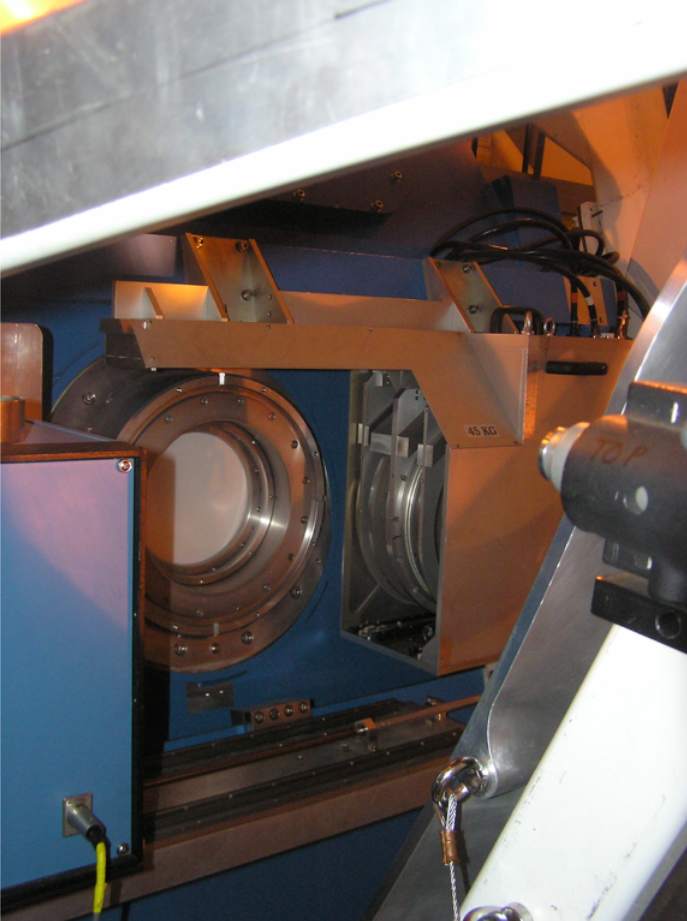
\includegraphics[width=0.45\linewidth]{pol2-out-of-beam.png}
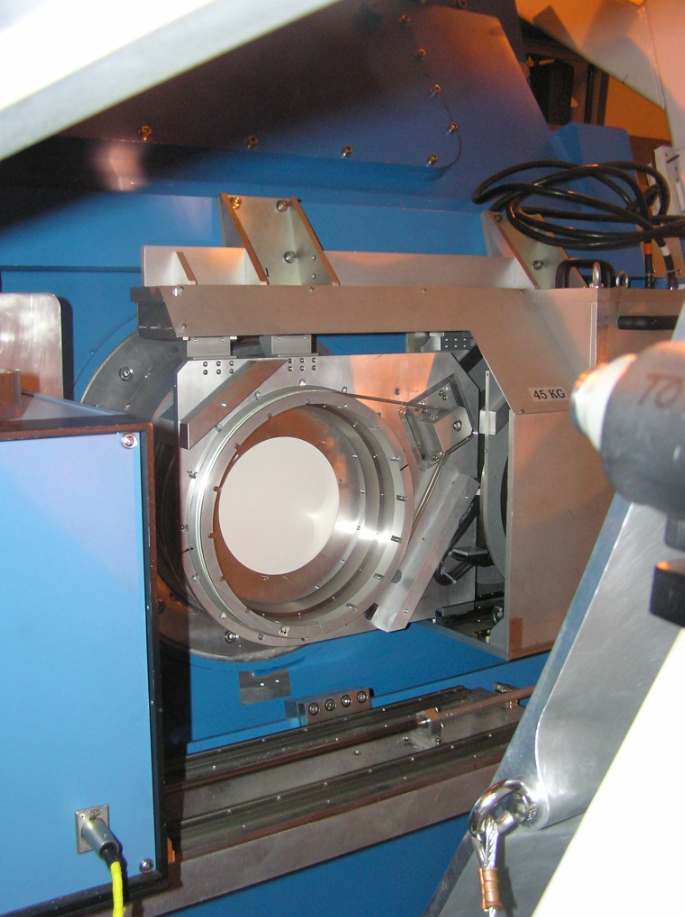
\includegraphics[width=0.45\linewidth]{pol2-in-beam.png}
\label{fig:pol2sc2}
\caption [POL-2 mounted on SCUBA-2]{POL-2 mounted on the front of
  SCUBA-2.  The left image shows the SCUBA-2 window. The right image
  shows the components of POL-2 inserted in front of the SCUBA-2
  window: the calibrator grid, rotating half-wave-plate (HWP) and the
  analyser grid. The calibrator grid is only inserted for test
  purposes.}
\end{center}
\end{figure}

\subsection*{Polarisation}

In polarimetric terms light is conventionally described by the four
Stokes parameters: $I$, $Q$, $U$ and $V$.


$I$ is the total intensity; $Q$ is the radiation linearly polarised in
the direction parallel or perpendicular to the reference plane. $U$ is
the radiation linearly polarised in the directions 45$^{\circ }$ to
the reference plane; and $V$ is the circularly polarised radiation.

POL-2 is designed to characterise linear polarisation.  The $V$
parameter, consequently, is not discussed further with the focus on $I$,
$Q$ and $U$.

The linear Polarised Intensity (I$_{p}$) and  polarisation angle
($\theta$) can be described as:

\begin{equation}
I_{p} = \sqrt{Q^{2}+U^{2}}
\end{equation}
\begin{equation}
\theta = 0.5\arctan(U/Q)
\end{equation}

with Q and U related to the polarisation angle and the polarised intensity by:

\begin{equation}
Q = I_{p} \text{cos}(2\theta)
\end{equation}
\begin{equation}
U = I_{p} \text{sin}(2\theta)
\end{equation}

where

\begin{equation}
Q = Q_{m} - I . IP_{q}
\end{equation}
\begin{equation}
U = U_{m} - I . IP_{u}
\end{equation}

where Q$_{m}$ and U$_{m}$ are the measured values of Q and U.  I is
the astronomical total intensity.  IP is the instrumental
polarisation. The IP affects both Q (\emph{via} IP$_{q}$) and U
(\emph{via} IP$_{u}$).


\subsection*{How POL-2 works}

POL-2 is located in front of the window to the SCUBA-2 instrument (as
is seen in Figure~\ref{fig:pol2sc2}), and covers the full field of
view of SCUBA-2. The POL-2 polarimeter uses three optical components
that cover the full field of SCUBA-2:

\begin{enumerate}
\item a wire-grid polariser used as a calibrator (only included in the
  beam for test purposes)
\item a Half-Wave Plate (HWP)
\item a second wire-grid polariser used as an analyser
\end{enumerate}

These components can be seen in Figure~\ref{fig:pol2sc2}.  A schematic
of POL-2 is given in Figure~\ref{fig:pol2sc2diagram}.

\begin{figure}[t!]
\begin{center}
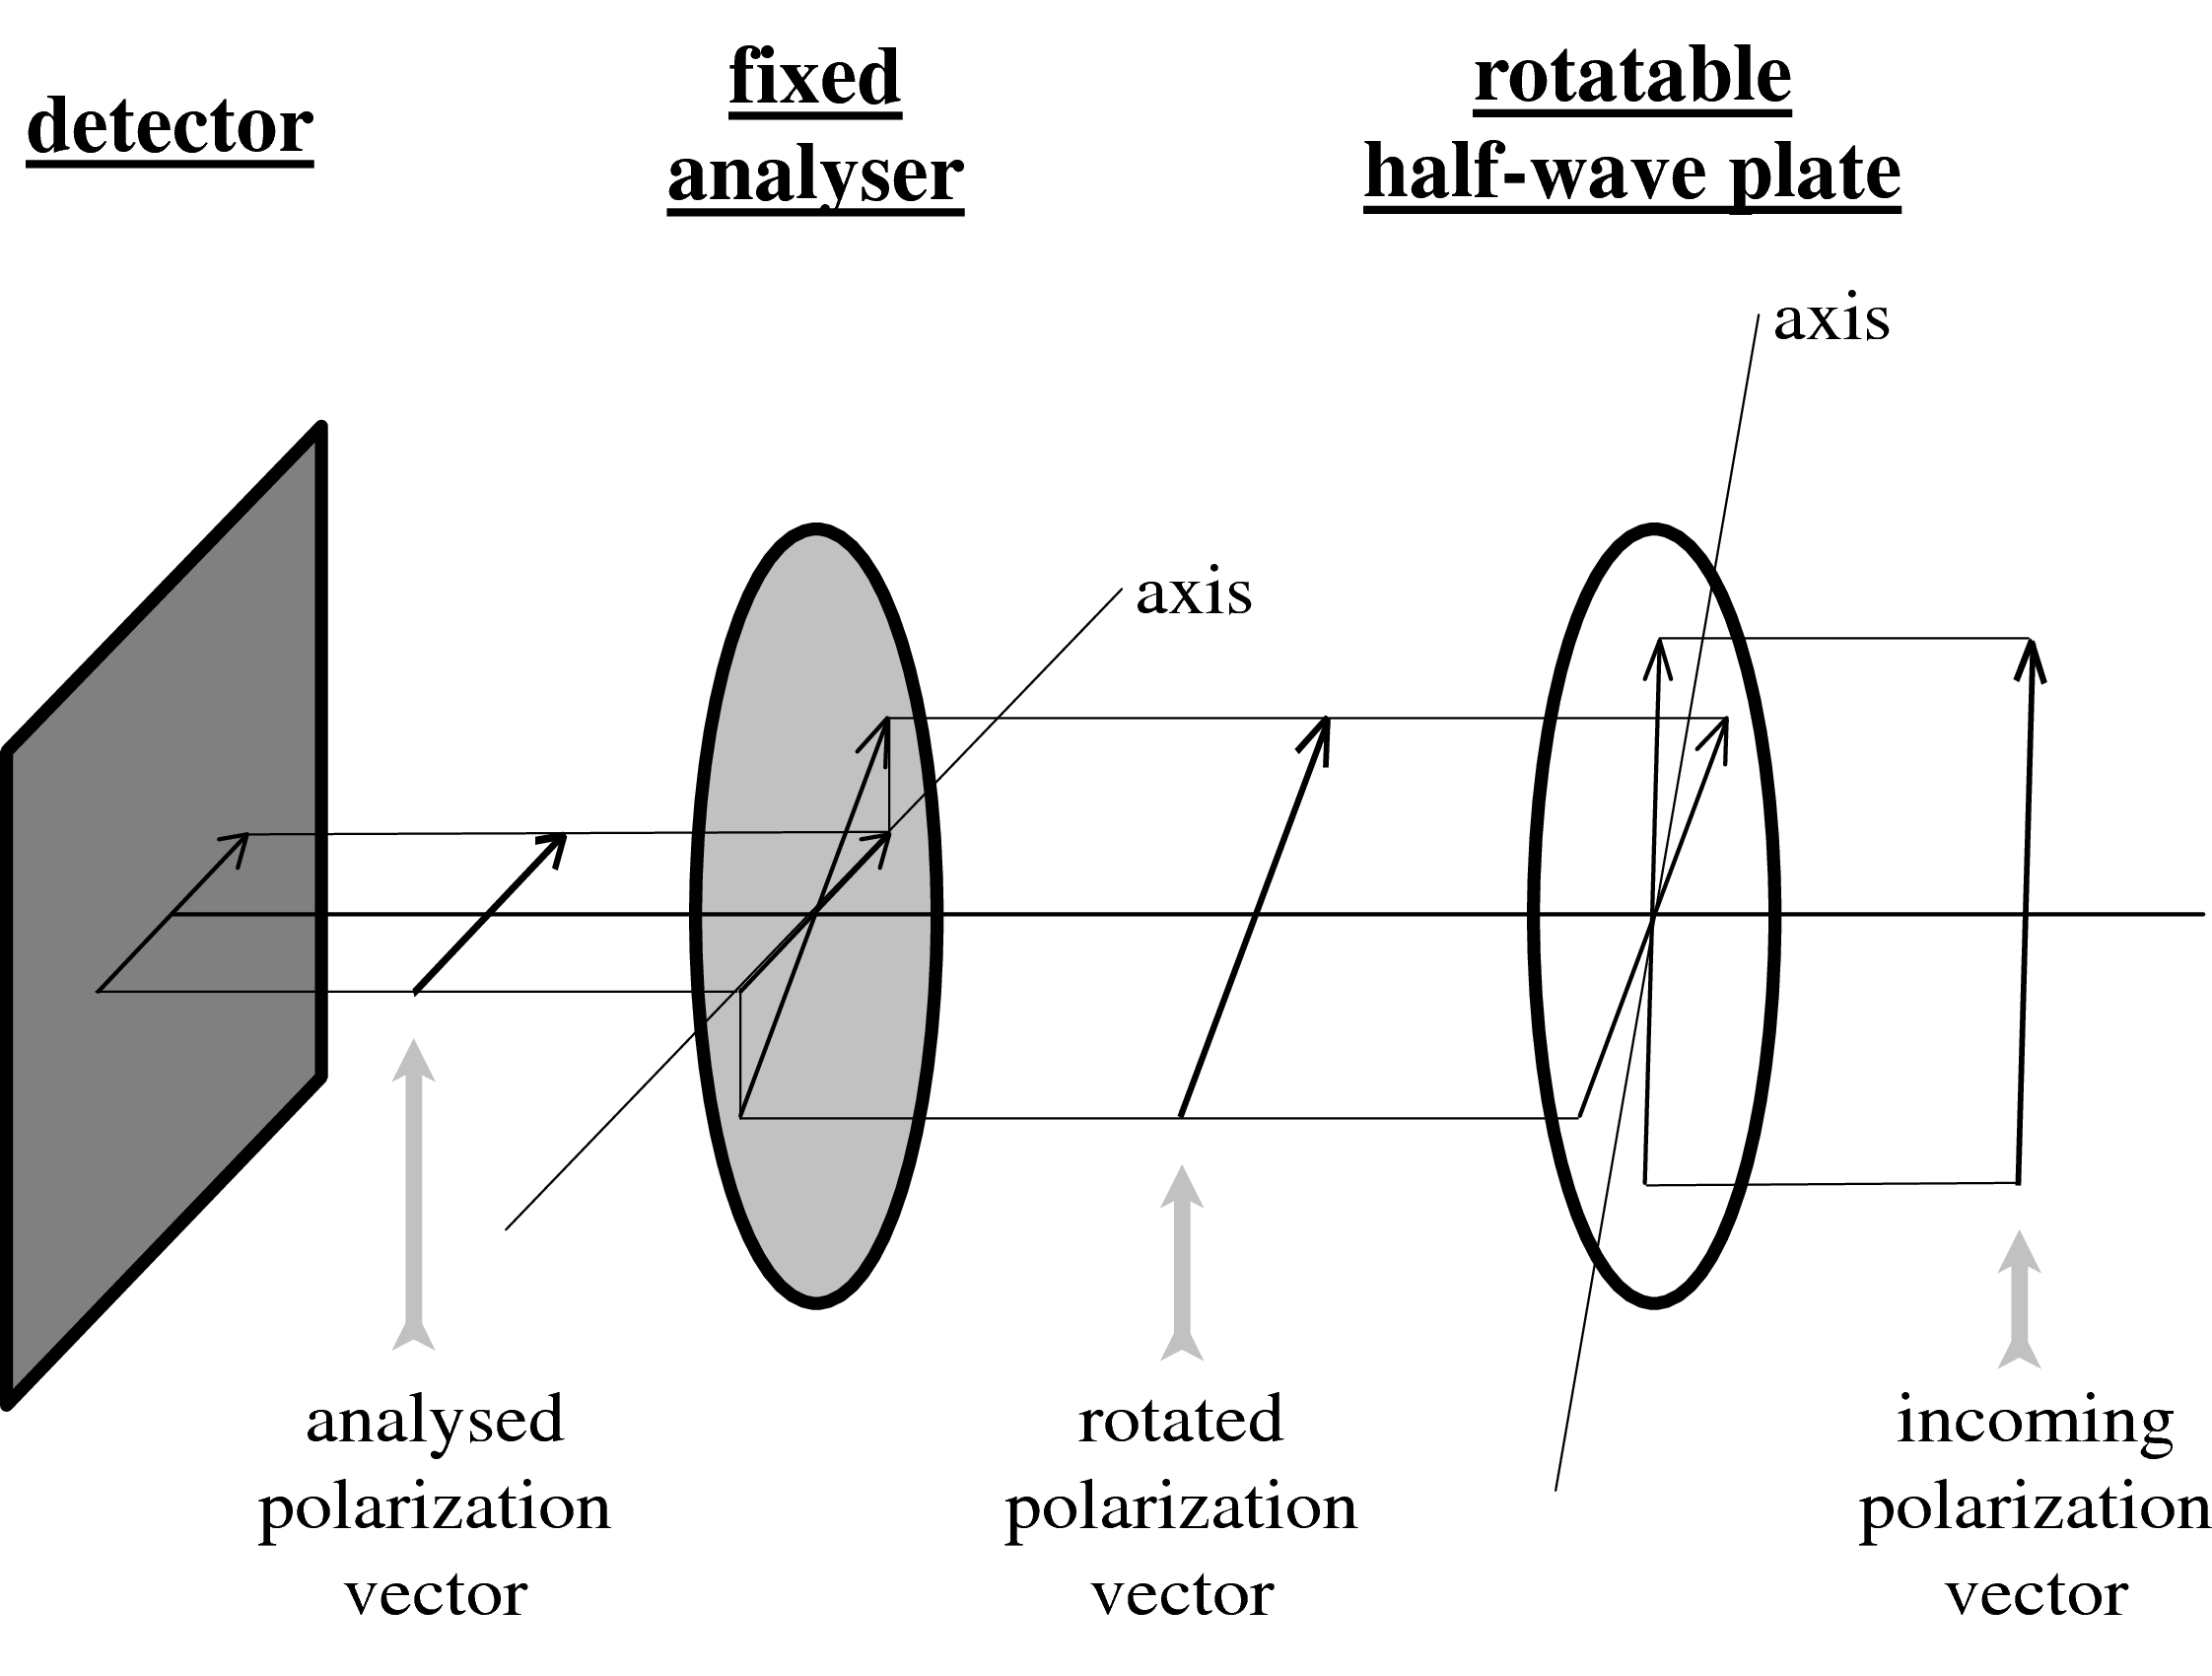
\includegraphics[width=0.8\linewidth]{singopt.png}
\caption [POL-2 optical components]{ The main optical components in a
  typical single-beam imaging polarimeter such as POL-2 (taken from
  SUN/223).}
\label{fig:pol2sc2diagram}
\end{center}
\end{figure}

Rotating the HWP rotates any linearly polarised component of incoming
radiation. The HWP rotates this incoming linear polarisation with
twice the speed of the HWP angle ($\delta$) producing the
\emph{effective analyser} position ($\phi$ - as defined in
\xref{the POLPACK documentation}{sun223} {thepolarimeter}), such that:


\begin{equation}
\phi = 2 \delta
\end{equation}


The rotating linearly polarised component is transmitted or reflected
by the grid, causing a modulation in the transmitted intensity.
The amplitude of the polarised component transmitted by the polariser is
$\sim$cos($\phi$) while the power is $\sim$cos$^{2}$($\phi$).

\begin{figure}[t!]
\begin{center}
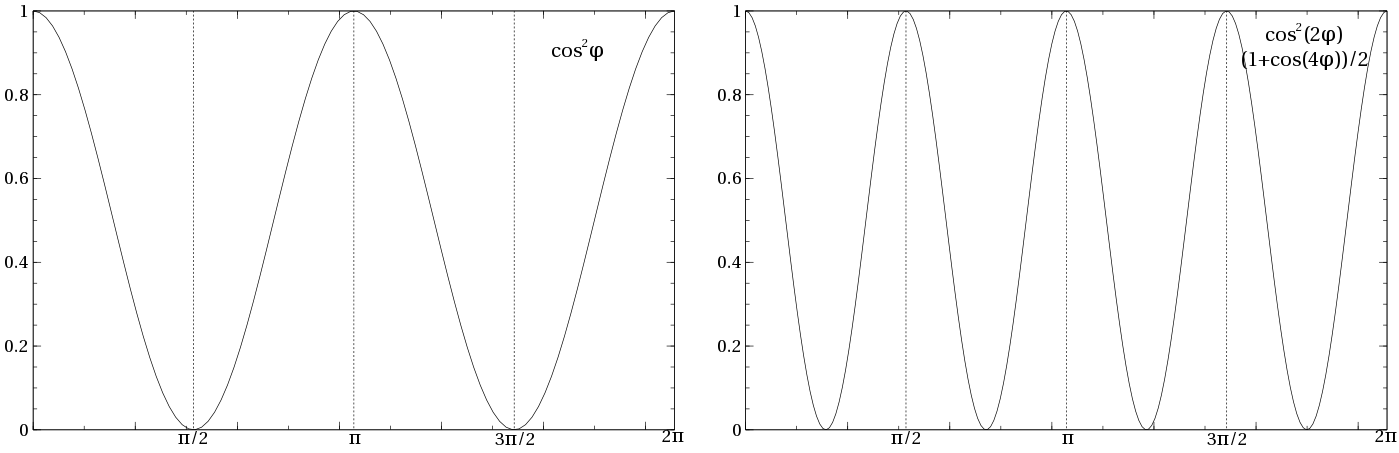
\includegraphics[width=0.95\linewidth]{hwp-modulation-basic.png}
\label{fig:hwp-modulation-basic}
\caption [Modulation by the HWP - basic description]{ Left: If there
  was a single rotating analyser this would be the resulting curve of
  the power transmitted of the linearly polarised component.
  Right: With the HWP the linearly polarised component is
  rotated at twice the speed. It may be useful to remind the reader of
  the trigonometric identity: \\ cos$^{2}$x = 0.5(1+cos(2x))}
\end{center}
\end{figure}


The radiation passing through the polarimeter is detected by
SCUBA-2. The detected intensity (I$_{detected}$) is a combination of
\emph{both} the unpolarised intensity (I$_{unpolarised}$) and the
linearly polarised intensity (I$_{p}$)\footnote{The total intensity of
the source, $I$, is $I_{unpolarised} + I_{p}$.}. This detected intensity can be
described by:

\begin{equation}
I_{detected} = \frac{I_{unpolarised}}{2}+ I_{p}\cdot\left(\frac{1+\cos(2\phi - 2\theta)}{2} \right)
\end{equation}

with the above equation being in terms of the effective analyser
angle, $\phi$ and the angle of the polarisation ($\theta)$.
This can also be expressed in terms of the  the HWP angle ($\delta$).

\begin{equation}
\label{eqn:idet}
I_{detected} = \frac{I_{unpolarised}}{2}+I_{p}\cdot\left(\frac{1+\cos(4\delta - 2\theta)}{2} \right)
\end{equation}




\subsection*{The Half-Wave Plate}

As described in the POL-2 commissioning document the HWP is
constructed from five individual synthetic sapphire layers
approximately 0.9 mm thick and 200 mm in diameter. The transmission
properties of sapphire are generally good at the SCUBA-2 wavelengths
but are dependent on the thickness and ambient temperature. The total
effective transmission of the HWP integrated across the 850 and
\SI{450}{\micro\metre} filter bands are about 86\% and 57\%
respectively (Savini et al. 2009 - insert full reference).

The HWP rotates the incoming linear polarisation with twice the speed
of the wave plate angle.  The HWP is typically rotated at 2Hz,
providing a fast modulation of any linear polarisation by 8Hz (see
equation~\ref{eqn:idet}).  The data acquisition rate is ~175Hz, yielding
20 samples per cycle.  The atmosphere is stable on the order of 2Hz and
can be removed.


\begin{figure}[t!]
\begin{center}
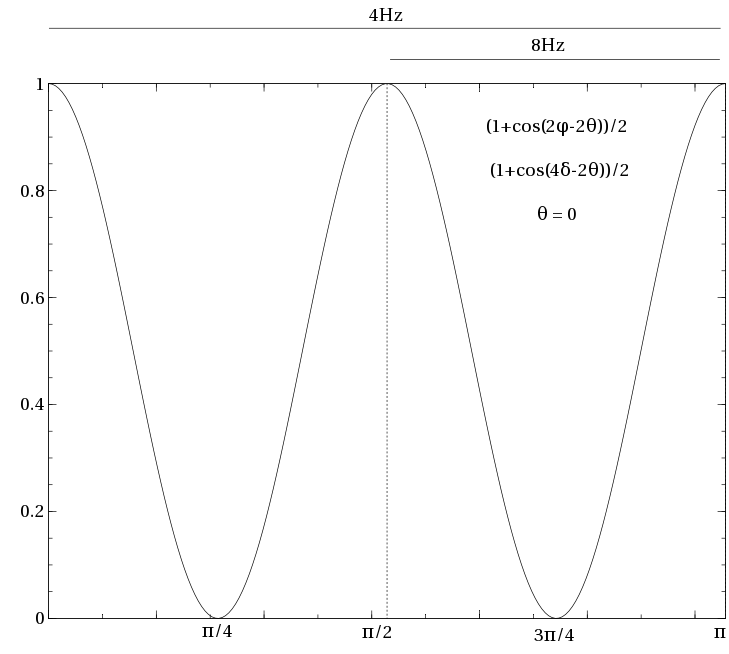
\includegraphics[width=0.7\linewidth]{hwp-modulation.png}
\label{fig:hwpmodulation}
\caption [Attenuation of signal by HWP]{The incoming polarised
  radiation (with a polarised angle, $\theta$, of zero) is attenuated
  by the HWP.  The HWP rotates at 2Hz (through $2\pi$) so we see the
  signal is modulated at 8Hz as the instrument scans at
  8\si{\arcsecond}/s. }
\end{center}
\end{figure}


\begin{figure}[t!]
\begin{center}
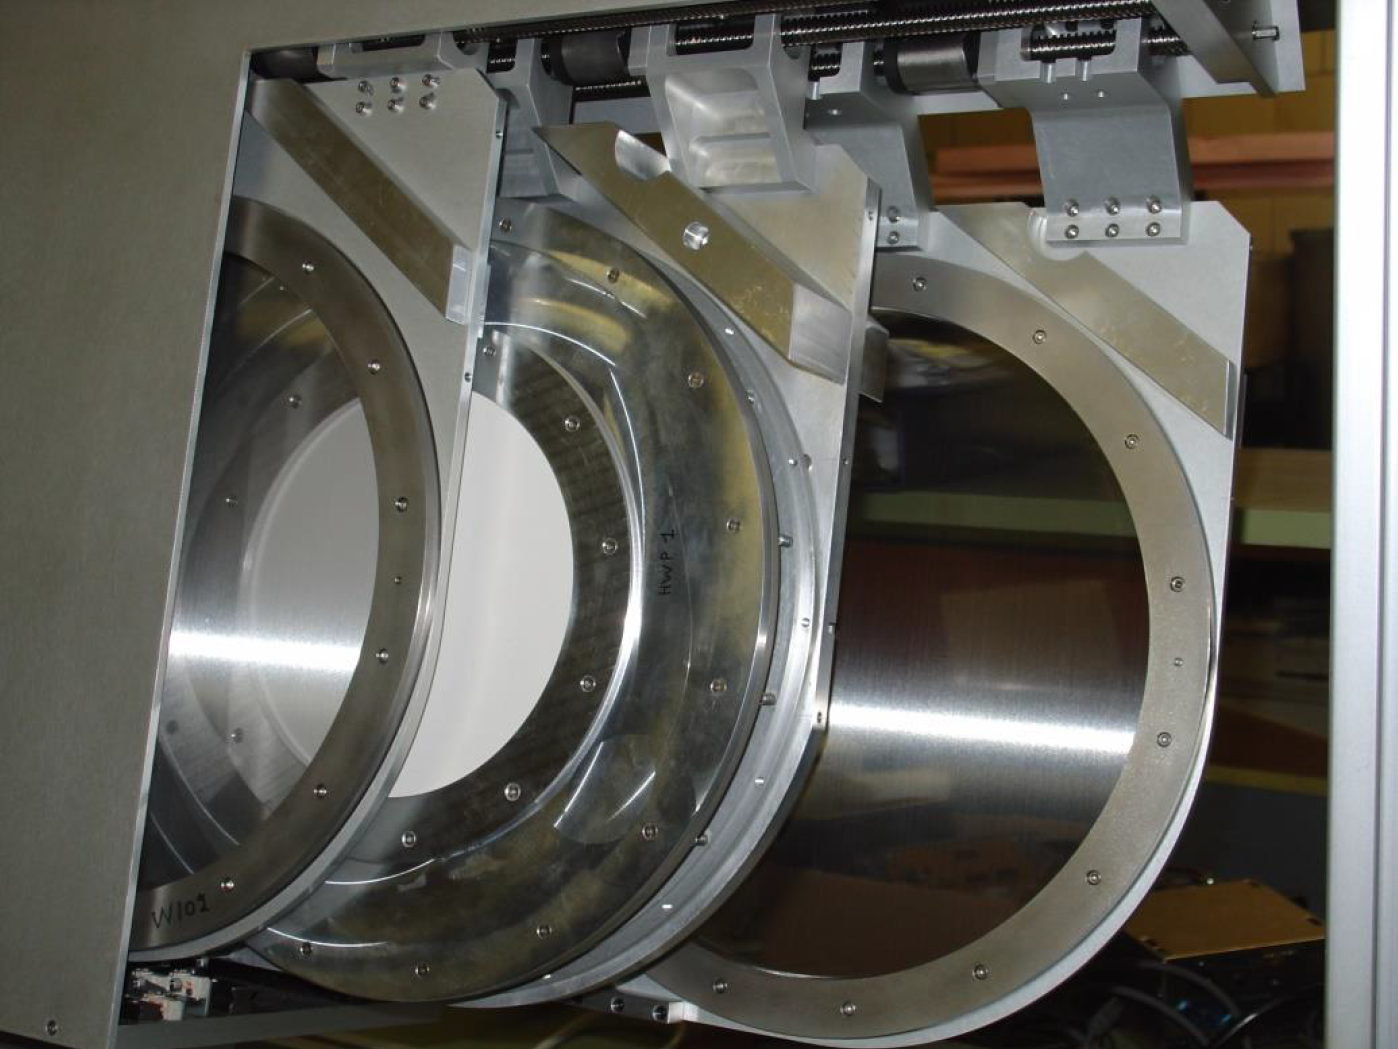
\includegraphics[width=0.7\linewidth]{pol2-three-components.png}
\label{fig:pol2components}
\caption [POL-2 components]{
  The three blades that combine to form POL-2 are partially
  extended showing the two wire grids and the achromatic HWP.
  The two wire grids are the calibrator grid and the analyser grid.
  The rotating HWP is located between these two fixed grids.
  The calibrator grid is only inserted for test purposes.
  Stiffeners can be seen on all three blades. The one for the HWP
  is particularly thick. Their purpose is to reduce vibrations while
  the HWP spins.
}
\end{center}
\end{figure}




\section{Instrumental Polarisation}
\label{sec:ip}

At the angular resolution of JCMT, planets such as Uranus should
appear as unpolarised point sources.  In practice, however, POL-2
observations of such sources exhibit a measurable level of
polarisation - albeit typically less than 1.5\% at 850 $\mu$m. This
is evidence that some part of the incoming astronomical radiation is
being partially polarised by one or more of the components of the
telescope/POL-2/SCUBA-2 that are in the light path. This polarisation
is referred to as "Instrumental Polarisation" (IP).

In order to establish the true Q and U from an astronomical source, it
is necessary to correct for this effect. For the case of a low degree
of polarisation in the incoming radiation and a low degree of IP, the
following is a good approximation for correcting the measurement for
the effects of the IP:

\begin{equation}
Q = Q_{m} - I. ip_{q}
\end{equation}

\begin{equation}
U = U_{m} - I. ip_{u}
\end{equation}

where $Q_{m}$ and $U_{m}$ are the measured values for a single
bolometer sample at some point on the sky. $Q$ and $U$ are the true
(corrected) values, $I$ is the astronomical total intensity at the same
point on the sky (i.e. the total intensity after removal of the sky
and electronic backgrounds) and $ip_{q}$ and $ip_{u}$ are factors that
may vary slowly with focal plane position and/or azimuth and
elevation.

IP correction of a POL-2 map therefore requires a total
intensity map of the same area of the sky to be available. This total
intensity map is referred to as the IP reference map.

Whilst flat mirrors or surfaces will produce a small, constant
polarisation across the beam, curved mirrors and other structures (for
example the secondary mirror supports) will produce more complex
polarisation effects, and these may distort the beam shape.
Side-lobes can often show up with strong (typically 10-20\%)
polarisation but these effects are usually far from the
main-beam. Calculations of typical antenna patterns for symmetrical
Cassegrain antennas have not predicted strong polarisation in the main
beam.

The JCMT IP footprint is stronger than might be expected from the
above considerations above (though typically less than 1.5\% of the
total intensity), and has the following distinctive features:

\begin{enumerate}
\item The polarisation intensity is elevation dependent;
\item There is ellipticity of the beam and it is elevation dependent;
\item The beam is elongated in the horizontal direction.
\end{enumerate}

The dominant source of IP at the JCMT is the woven Goretex membrane,
used as a wind blind.  This membrane introduces both losses and
polarisation. This effect is elevation dependent.


\section{\xlabel{obs_modes}Observing mode}
\label{sec:mmodes}

The standard POL-2 observing mode, POLCV\_DAISY, is a “scan and spin”
mode, in which the telescope is moving continuously in a Daisy-type
pattern while the HWP spins.

The POLCV\_DAISY scan mode is similar to the established Daisy scan
mode routinely used for non-polarimetric SCUBA-2 observations of
point-like or compact sources. However it is slightly altered to allow
for a slower telescope scanning speed.


\begin{figure}[t!]
\begin{center}
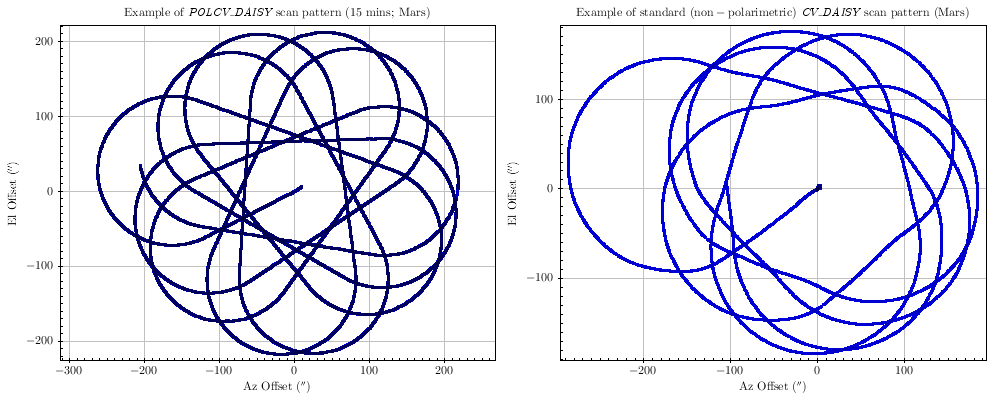
\includegraphics[width=0.9\linewidth]{scan_pattern_daisy_comparison.png}
\label{fig:scancompsrison}
\caption [Scan Pattern Comparison]{Left: Scan pattern from a typical
  SCUBA-2 CV\_Daisy observation. Right: Scan pattern from a POL-2
  Daisy. The standard POLCV\_DAISY scan parameters are given in Table
  \ref{tab:scanpar} }
\end{center}
\end{figure}


The telescope must scan slowly enough to obtain sufficient data at
each point on the sky to allow good $Q$ and $U$ values to be
determined. The current commissioned scan pattern has a size of
200\si{\arcsecond} and a scan speed of 8\si{\arcsecond}/s. The data
reduction splits the data stream into short segments and determines a
pair of $Q$ and $U$ values from each segment.

The length of each such data segment is the time it takes the
telescope to traverse a pixel in the generated map. With the current
scanning parameters this is 0.5 and 0.25 seconds for 850 and
\SI{450}{\micro\metre}, respectively. The modulation generated by any
polarisation is 8 Hz at the current HWP rotation speed (2 Hz).

The standard POLCV\_DAISY scan parameters are given in
Table~\ref{tab:scanpar} and shown in Figure~\ref{fig:scandetail}.

\begin{table}[h!]
\begin{center}
\begin{tabular}{r|l}
\hline
Parameter & Value\\
\hline
Half-wave plate rotation frequency& \SI{2}{Hz}\\
 Antenna scanning speed & 8\si{\arcsecond}/s\\
 R$_{0}$ (map pattern radius)\textdagger
& 133\si{\arcsecond}\\
 R$_{t}$ (turn radius) & 99\si{\arcsecond}\\
 R$_{a}$ (nominal avoidance radius) & 77\si{\arcsecond}\\
\hline
\end{tabular}
\caption{The scan parameters used in the POLCV\_DAISY
  mode. \textdagger This radius is \emph{not} the size of the
  resulting map. }
\label{tab:scanpar}
\end{center}
\end{table}


\begin{figure}[t!]
\begin{center}
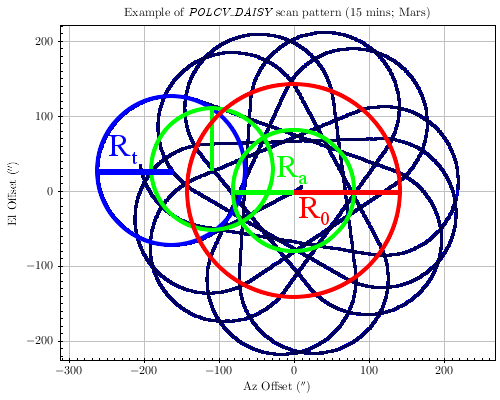
\includegraphics[width=0.6\linewidth]{POLCV_DAISY_schematic_detailed.png}
\caption [Detail of POL-2 Scan Pattern]{Detail of
  POLCV\_DAISY. $R_{0}$ is the map pattern radius, $R_{t}$ the turn
  radius, and $R_{a}$ is the nominal avoidance radius. For more
  details see Table~\ref{tab:scanpar}.}
\label{fig:scandetail}
\end{center}
\end{figure}


\section{The raw data}
\label{sec:rawdata}
SCUBA-2 is the detector for POL-2, and as such, the raw data format of
POL-2 data is the same as a typical SCUBA-2 observation. The sequence
for both observations is:

\begin{enumerate}\itemsep-0.2em
\item Dark noise
\item Flat-field
\item Science scans
\item Flat-field
\end{enumerate}


The \param{SEQ$\_$TYPE} keyword in the FITS header may be used to
identify the nature of each scan.  When you access raw data from the
CADC archive
\htmladdnormallink{http://www3.cadc-ccda.hia-iha.nrc-cnrc.gc.ca/jcmt/}\
you will get all of the files listed above.


Critically the \param{INBEAM} keyword in the FITS header may be used
to identify if POL-2 is in the beam, and hence differentiate between
SCUBA-2 and POL-2 observations.


\begin{tip}
  Use the \Kappa\ command fitslist to see all FITS headers in a
  particular NDF. To obtain a specific header simply use the command
  fitsval:
  \begin{terminalv}
% fitsval s8a20160112_00056_0001.sdf INBEAM
pol
\end{terminalv}
The FITS header information may also be viewed via the \gaia\ View /
FITS header drop-down menu option.
\end{tip}

Shown below is an incomplete list of the raw files for a single
sub-array (in this case s8a) for a short POL-2 observation. The first
and last scans are the flat-field observations,which occur after the
shutter opens to the sky at the start of the observation and closes at
the end (note the identical file size); all of the scans in between
are science scans.


\begin{terminalv}
% ls -lh /jcmtdata/raw/scuba2/s8a/20160112/00056
\end{terminalv}

\begin{terminalv}
-rw-r--r-- 1 jcmtarch jcmt 5.6M Jan 12  2016 s8a20160112_00056_0001.sdf
-rw-r--r-- 1 jcmtarch jcmt 7.9M Jan 12  2016 s8a20160112_00056_0002.sdf
-rw-r--r-- 1 jcmtarch jcmt  25M Jan 12  2016 s8a20160112_00056_0003.sdf
-rw-r--r-- 1 jcmtarch jcmt  25M Jan 12  2016 s8a20160112_00056_0004.sdf
-rw-r--r-- 1 jcmtarch jcmt  25M Jan 12  2016 s8a20160112_00056_0005.sdf
...
-rw-r--r-- 1 jcmtarch jcmt  25M Jan 12  2016 s8a20160112_00056_0025.sdf
-rw-r--r-- 1 jcmtarch jcmt  25M Jan 12  2016 s8a20160112_00056_0026.sdf
-rw-r--r-- 1 jcmtarch jcmt  25M Jan 12  2016 s8a20160112_00056_0027.sdf
-rw-r--r-- 1 jcmtarch jcmt  22M Jan 12  2016 s8a20160112_00056_0028.sdf
-rw-r--r-- 1 jcmtarch jcmt 7.9M Jan 12  2016 s8a20160112_00056_0029.sdf
\end{terminalv}

The SCUBA-2 data acquisition (DA) system writes out a data file every
30 seconds; each of which contains 22\,MB of data. The only exception
is the final science scan which will usually be smaller (7.9\,MB in
the example above), typically requiring less than 30 seconds of data
to complete the observation.

\textbf{Note:} All of these files are written out eight times, once
for each of the eight sub-arrays. It should also be noted that the
POL-2 instrument has not been released from commissioning at 450
$\mu$m.

The main data array in each NDF is a cube, with the first two
dimensions corresponding to bolometer columns and rows within a
sub-array, and the third dimension corresponding to time slice index
(sampled at roughly 200\,Hz).

A standardised file naming scheme is used in which each file name
starts with the sub-array name, followed by the UT date of the
observation in the format \texttt{yyyymmdd}, followed by a five-digit
observation number, followed by the sub-scan number. The name ends
with the standard suffix \texttt{.sdf} used by all Starlink NDF data
files. For instance, the files listed above hold data from the s8a
sub-array for observation 34 taken on 12\textsuperscript{th} January
2016.




\subsubsection*{Units/Calibration}

Raw POL-2 data come in uncalibrated units. The first calibration step
is to scale the raw data to units of pico Watts (pW) by applying the
flat-field solution. This step is performed internally by the SMURF
command calcqu - used to calculate I, Q and U time-streams from the
raw data - but can be done manually when examining the raw data.

If the purpose of a given POL-2 observation is to determine the
percentage polarisations or vector angles within a source/region of
interest then the data may remain in pW. On the other hand, if the
purpose is to establish the absolute polarised intensities then a
value for the Flux Conversion Factor (FCF) is required.

The resulting map may have the FCF applied to convert it into units of
Janskys. As is recommended with SCUBA-2 observing, it is advisable to
check that the FCF value applied to the data is sensible (and must be
done manually). For more details see
\cref{Chapter}{sec:pol2map-fcf}{POL-2 FCFs}.






\newpage
\chapter{\xlabel{pol2_dr}POL-2 Data Reduction - The Theory}
\label{sec:dr}
\section{\xlabel{dataflow}The Data Flow}

POL-2 data reduction is a complex and involved process for which a broad overview is presented first before
the specific details are discussed. It is noted that this same procedure is used whether there is one or 
multiple observation to reduce.

The data reduction process can be broken down into three main steps as shown in Figure \ref{fig:pol2drflow}.

\begin{figure}[t!]
\begin{center}
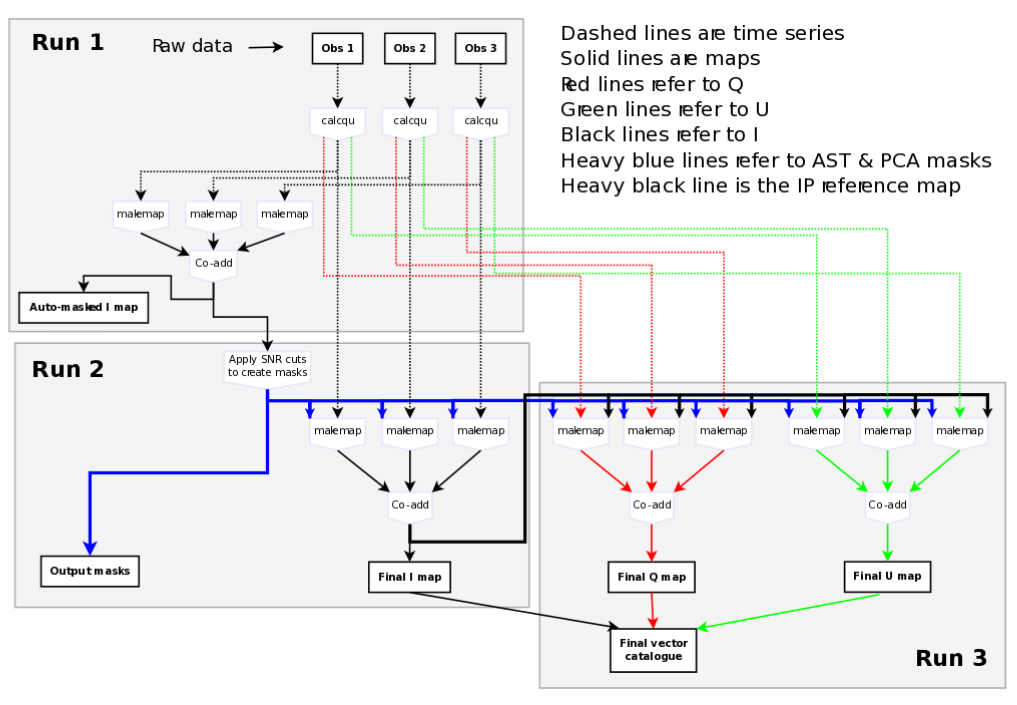
\includegraphics[width=0.95\linewidth]{pol2-dr-flow.png}
\label{fig:pol2drflow}
\caption [POL-2 Data Flow]{
  \small The data flow of the POL-2 data reduction method is
  presented. In this example three POL-2 observations are
  reduced and combined in various stages and combination to
  produce I, Q and U maps.
}
\end{center}
\end{figure}


\subsection*{Step 1}

The inital step of the process (see Run 1 in Figure \cite{fig:pol2drflow}) creates 
an intensity, I, map from the raw data files provided to the reduction routine (see \cref{Chapter}{sec:rundr}). 


\subsubsection*{The process}
The  analysed  intensity values in the raw data time-streams are first converted into Q, U and I time-streams
using smurf:calcqu (these are stored for future use in the directory qudata, specified by the qudir parameter in the example command below). 

The smurf:makemap command is then used to create a separate map from the I time-stream for each observation, using SNR-based “auto-masking” to define the background regions that are to be set to zero at the end of each iteration.  

These maps are stored for future use in the directory maps, specified by the mapdir parameter. Each map has a name of the form:

<UT_DATE>_<OBS_NUM>_<CHUNK_NUM>_imap.sdf

where <CHUNK_NUM> indicates the raw data file at the start of the contiguous chunk of data used to create the map, and is
usually 0003. Each of these maps is compared to the specified reference map (if any) to determine a pointing correction to be applied to the observation in future
2 . If no reference map is supplied, the I map created from the first observation defines the expected source position, and is compared with later maps to determine their pointing corrections.


\subsection*{Step 2}

In the second step of the process (see Run 2 in Figure \cite{fig:pol2drflow}) an improved I map is produced. This improvements come from i) applied relative pointing corrections 


\subsection*{Step 3}



\section{\xlabel{makemap}Makemap}

The POL-2 data reduction builds upon the SCUBA-2 make-map data reduction. The Dynamic Iterative Map-Maker, hereafter just referred to as the map-maker is the tool you will use to produce SCUBA-2 maps, and is implemented by the Smurf makemap command. It performs all pre-processing steps to clean the data, followed by solving for multiple signal components using an iterative algorithm, and binning the resulting time-series data to produce a final science map. 



\cite{smurf}

\section{\xlabel{pca}PCA}


\section{\xlabel{masking}Masking}
A mask is a two-dimensional array which has the same shape and size as the final map, and
which is used to indicate where the source is expected to fall within the map. Bad pixel values
within a mask indicate background pixels, and good pixels values indicate source pixels. Masks
are used for two main purposes:

\begin{enumerate}\itemsep-0.2em
\item To prevent the growth of gradients and other artificial large scale structures within the
map.  For this purpose, the astronomical signal at all background pixels defined by the
mask is forced to zero at the end of each iteration within makemap (except for the final iteration).
\item To prevent bright sources polluting the evaluation of the various noise models (PCA, COM, FLT) used within
makemap. Source pixels are excluded from the calculation of these models.
\end{enumerate}


The pol2map script uses different masks for these two purposes - the “AST” mask and the “PCA” mask. 
The PCA mask is in general less extensive than the AST mask, with the source areas being restricted to the brighter inner regions.
Each of these two masks can either be generated automatically within makemap, or be specified by
a fixed external NDF. 

\section{\xlabel{addingdata}Adding new observations}



\section{\xlabel{tailoredDR}Tailoring your reduction}

\subsection*{variances between POL-2 maps}

MAPVAR is a parameter that controls the variances in the coadded 
I, Q and U maps are formed.

If  MAPVAR is set TRUE, the variances in the coadded I, Q and U maps
are formed from the spread of pixel data values in the individual
observation maps. If MAPVAR is FALSE (the default), the variances in
the coadded maps are formed (as in previous versions of pol2map) by
propagating the pixel variance values created by makemap from the
individual observation maps.

Only use MAPVAR=TRUE if you have enough observations to
make the variances between them meaningful. It's hard to put a lower
limit on it, but it is advised that at a minimum 10 observations.


If you want to test the effect of this option on a field for which you
already have the I, Q and U maps from a set of individual
observations, you can do the following:

\begin{terminalv}
% pol2map in=maps/\* iout=imapvar qout=qmapvar uout=umapvar mapvar=yes \
                   ipcor=no cat=cat_mapvar debias=yes
\end{terminalv}

assuming your I, Q and U maps are in directory "maps". The variances
in imapvar.sdf qmapvar.sdf and umapvar.sdf will be calculated using
the new method, and these variances will then be used to form the
errors in the cat_mapvar.FIT catalogue.





\begin{thebibliography}{}
\addcontentsline{toc}{section}{References}




\bibitem{archibald}
Archibald,~E.~N., et~al, 2002, \htmladdnormallink{\textit{On the atmospheric limitations
of ground-based submillimetre astronomy using array receivers}}{http://dx.doi.org/10.1046/j.1365-8711.2002.05582.x}, MNRAS, 336, 1-13
(DOI:10.1046/j.1365-8711.2002.05582.x)

\bibitem{fellwalker}
Berry~D.~S.,  2015,
\htmladdnormallink{\textit{FellWalker - a Clump Identification Algorithm}}
{http://dx.doi.org/10.1016/j.ascom.2014.11.004},
Ast. \& Comp., 10, 22-31 (DOI:10.1016/j.ascom.2014.11.004)

\bibitem{oracdr}
Cavanagh~B., Jenness~T., Economou~F., Currie~M.~J., 2008,
\htmladdnormallink{\textit{The ORAC-DR data reduction
pipeline}}{http://dx.doi.org/10.1002/asna.200710944}, Astron. Nactr., 329, 295
(DOI:10.1002/asna.200710944)

\bibitem{smurf}
Chapin~E.~L., et~al., 2013, \textit{SMURF -- Sub-Millimetre User Reduction
Facility}, \xref{Starlink User Note 258}{sun258}{}

\bibitem{mapmaker}
Chapin~E.~L., et~al., 2013,
\htmladdnormallink{\textit{SCUBA-2: iterative map-making with the
Sub-Millimetre User Reduction Facility}}{http://dx.doi.org/10.1093/mnras/stt052},
MNRAS, 430, 2545 (DOI:10.1093/mnras/stt052)

\bibitem{ssds}
Currie~M.~J., Wallace~P.~T., Warren-Smith~R.~F., 1989,
\textit{Starlink Standard Data Structures}, \xref{Starlink General
Paper 38.2}{sgp38}{}

\bibitem{kappa}
Currie~M.~J., Berry~D.~S, 2013, \textit{KAPPA -- Kernel Application Package},
\xref{Starlink User Note 95}{sun95}{}

\bibitem{dempsey12}
Dempsey~J.~T. et al., 2013, \htmladdnormallink{\textit{SCUBA-2: on-sky calibration using
submillimetre standard sources}}{http://dx.doi.org/10.1093/mnras/stt090},
MNRAS, 430, 2534 (DOI:10.1093/mnras/stt090)

\bibitem{dempsey-spie}
Dempsey~J.~T., Friberg~P., Jenness~T., Bintley~D., Holland~W.~S., 2010
\htmladdnormallink{\textit{Extinction correction and on-sky calibration of
SCUBA-2}}{http://dx.doi.org/10.1117/12.856476},
Proc.\ SPIE, 7741 (DOI:10.1117/12.856476)

\bibitem{gaia}
Draper~P.~W., Gray~N., Berry~D.~S., Taylor~M., 2012,
\textit{GAIA -- Graphical Astronomy and Image Analysis Tool},
\xref{Starlink User Note 214}{sun214}{}

\bibitem{picard}
Gibb~A.~G., Jenness~T., Economou~F., 2012, \textit{PICARD --- a
PIpeline for Combining and Analyzing Reduced Data}
\xref{Starlink User Note 265}{sun265}{}

\bibitem{s2main}
Holland, W. S., et~al, 2013, \htmladdnormallink{\textit{SCUBA-2: The
10,000 pixel bolometer camera on the James Clerk Maxwell Telescope}}
{http://dx.doi.org/10.1093/mnras/sts612}, MNRAS, 430, 2513
(DOI:10.1093/mnras/sts612)

\bibitem{flux1}
Jenness~T., et~al, 2002, \htmladdnormallink{\textit{Towards the automated
reduction and calibration of SCUBA data from the James Clerk Maxwell
Telescope}}{http://dx.doi.org/10.1046/j.1365-8711.2002.05604.x},
MNRAS, 336, 14-21 (DOI:10.1046/j.1365-8711.2002.05604.x)

\bibitem{ndf}
Jenness~T., et~al, 2014,
\htmladdnormallink{\textit{Learning from 25 years of the extensible
N-Dimensional Data Format}} {http://dx.doi.org/10.1016/j.ascom.2014.11.001},
Ast. \& Comp., in press, (DOI:10.1016/j.ascom.2014.11.001)

\bibitem{Friberg}
Friberg,~P., et~al, 2016 \htmladdnormallink{\textit{POL-2: a polarimeter 
for the James-Clerk-Maxwell telescope}}{http://proceedings.spiedigitallibrary.org/proceeding.aspx?articleid=2536885},
SPIE, Volume 9914, id. 991403
(DOI: 10.1117/12.2231943)

\bibitem{sc2ana005}
Scott~D., Van Engelen~A., 2005, \htmladdnormallink{\textit{Scan Mode Strategies for
SCUBA-2}}{http://docs.eao.hawaii.edu/JCMT/SC2/ANA/S210/005/sc2_ana_s210_005.ps},
SCUBA-2 Data Reduction document SC2/ANA/S210/005

\end{thebibliography}

\newpage
\appendix
\chapter{\xlabel{pca_scuba2}PCA on SCUBA-2 data}
\label{app:pca}

This document has outlined the process of reducing POl-2 data and its
reliance on PCA during the makemap process.There are two main reasons 
why runnign makemap with PCA is not the default method for all data observed
using SCUBA-2. 

\begin{enumerate}
\item It is time consuming to run
\item Produces similar results to running the default makemap as 
is obtained by simply increasing the filter size.
\end{enumerate}

The tools however are still provided and so those wo are interested
may use this method to compare results.




\end{document}

